\chapter{Context}

% Starting with summarizing and then explanation of those concepts
To fully understand the ideas behind this thesis and results which can be achieved we need to delve deeper into two key areas: DOTS and GGPO. DOTS encompasses a spectrum of concepts ranging from games and game engines to performance and scalability issues, along with the principles of Data-Oriented Design (DOD). On the other hand, understanding GGPO consist of familiarity with various types of netcodes and a comprehensive grasp of what GGPO specifically is. This thorough exploration will provide the foundation necessary for comprehending the thesis and its implications.\newline

% Introduction of gaming in general and why its worth researching
We will start with broad introduction to gaming and it's ever-evolving environment which stands as the core of this thesis and which continuously adapts alongside technological progressions and shifting player preferences. Originating from humble beginnings with arcade machines, gaming has transformed into the extended virtual worlds of today, spanning diverse platforms and genres. The gaming industry has transitioned into a formidable cultural and economic force, surpassing its conventional perception as a solely form of entertainment. Instead, it has emerged as an influential medium in art, education, and social interaction. Consequently, the necessity to research and innovate within the gaming domain extends beyond conventional boundaries, encompassing diverse fields of study and application.\newline

% Introduction of multiplayer games and lag+cpu usage (the problem)
Within this environment, multiplayer experiences stand out as among the most complicated to develop, requiring a blend of techniques to seamlessly synchronize real-time interactions among players. Unlike single-player or local multiplayer games, where actions are confined to a single system, the complexity escalates with multiple players, amount of events happening in the scene at once, varied network conditions, and the inherent uncertainties of data transmission. As players expect immersive and uninterrupted gaming experiences, especially in scenarios with numerous entities seamlessly interconnected globally, two primary challenges emerge: CPU processing and network latency. The first one encompasses problems related to handling a lot of entities at the same time in bigger and bigger game worlds which ideally should also run on devices with not top hardware, when also in need to apply remote changes of other players and occasionally having to simulate several frames in the timespan of one to catch up with the game state. The other issue of latency which is the delay encountered in transmitting data over the internet and delivering it seemlesly on time, influenced by factors such as geographical distance, network congestion, and computational capabilities which can hinder even the best in other aspects games. This latency and computational load can impede players from fully enjoying expansive games, disrupting gameplay flow and diminishing overall enjoyment, underscoring the critical need for effective strategies to mitigate latency especially in combination with games with high CPU usage.\newline

% Introduction of netcode strategies
When understanding the general problem we will explore first the netcode itself and its means to mitigate network latency. Before the first appearance of rollback netcode solutions in 1996 used by GGPO, online gaming predominantly relied on delay-based systems. These systems aimed for perfect synchronization between players, requiring both parties to wait for each other's inputs before advancing the game to the next frame. Unfortunately, this often led to frustrating freezes and missed inputs due to network challenges. The deeper explanation of how it works can be find here: \cite{Delaybased_rollback_explanation}.

% Introduction of rollback netcode
In contrast, rollback netcode especially in combination with and player prediction revolutionized online gaming with its approach, addressing the challenges of latency in fast-paced games where player reaction windows can be as narrow as 100 milliseconds (With the round trip time of many network connections stretching into 200-500 ms of latency). Rollback netcode attempts to remedy this with speculative execution: it attempts to predict remote inputs (when latency prevent them to arrive on time) based on prior inputs and roll back and replay the simulation only when necessary. This allows games to continue simulation as if the game were entirely local. Rollback netcode ensures that players experience minimal disruptions (players only notice the network latency if the predictions are wrong), making for a much smoother online experience, particularly crucial in fast-paced competitive genres like fighting games or real-time strategy (RTS) titles, where split-second reactions can determine victory or defeat. The summary of it can be find here: \cite{Rollback_overview}. "Rollback networking" is a vague term describing any form of data rollback + resimulation. GGPO and N4E models both do rollback and resimulation, thus they are both "rollback networking" architectures. The differences between the two architectures is more to do with how they synchronise (i.e. replicate) entities.

There are only a few different types of Netcode architecture, but almost every game will have a unique implementation of one of these architectures. We're using the GGPO architecture (or model) because: Determinism and lockstep allows you to:
Only replicate inputs, leading to extremely low bandwidth consumption.
Synchronise an enormous number of entities easily.
Write the gameplay code without having to care much about latency or netcode concepts.
Get anti-cheat in a "peer to peer" (and/or Relay) environment, without the need for expensive dedicated game servers.
The "Rollback and resimulation" feature gives you the ability to hide most of the latency that exists in Lockstep architectures.\newline

% Introduction of GGPO, would necessary 
At the forefront of this shift was GGPO (Good Game Peace Out) which is one of the two core concepts in this thesis. It was a pioneering networking framework that introduced rollback netcode with lockstep and player prediction in late 2006. The GGPO networking SDK is designed to facilitate the seamless incorporation of rollback networking into both new and existing games. Furthermore, in 2019, the framework transitioned to an MIT license, making it accessible to a wider range of developers. Despite its age, GGPO remains a cornerstone in online gaming infrastructure, with many games still utilizing its capabilities to provide supreme online experiences explained at their website \cite{GGPO_page}. For the sake of this thesis a custom implementation of GGPO will be implemented because it will give us more flexibility, potentially easier implementation. GGPO fundamentally is just taking a Deterministic Lockstep architecture (like Age of Empires 2) and adding rollback + resimulation to it. (client prediction?)
Client prediction (a.k.a. rollback and resimulation) in an "Eventual Consistency" "Client & Server" "Snapshot Synchronization" netcode model (NetCode for Entities can be described as all of these) is useful for hiding latency.
Similarly, Client prediction (a.k.a. rollback and resimulation) in an "Deterministic Lockstep" "P2P/Relay" netcode model is useful for hiding latency.
In other words: We're not trying to "improve" prediction here, GGPO offers another approach to handling NetCode in a game, which is more suitable for some game genres (RTS & Fighting).
\newline

% Introduction of gaming engines
After explenation of one of the core aspects of the thesis which is GGPO now we need to delve deeper into exploration what DOTS actually is. Behind this concept stands Unity which is one of the most popular gaming engines. Game engine in its core serves as the foundation upon which video games are built. Gaming engines provide developers with a comprehensive suite of tools and functionalities to create games efficiently. These engines encompass various software components, handling tasks such as rendering graphics, managing audio, simulating physics, and implementing artificial intelligence. By utilizing pre-built systems and libraries within the gaming engine, developers can streamline the development process, focusing more on designing gameplay mechanics and content rather than reinventing the wheel. Additionally, gaming engines often offer cross-platform compatibility, enabling games to be deployed across different devices and operating systems with minimal modifications. In essence, a gaming engine acts as the backbone of game development, empowering developers to bring their creative visions to life with efficiency and flexibility. Some notable examples include Unity, Unreal, Godot, and CryEngine described more in details here: \cite{Game_engines_comparison}. While some companies develop their own proprietary engines, many developers, especially indie game developers, find it easier to leverage existing solutions and that's why they would gain the most from integration of new technoques and systems into the game engine that they are using.\newline

% Introduction of UNITY
Among the array of gaming engines available, Unity stands out as one of the most prominent and versatile options in the industry. Renowned for its accessibility, Unity offers a robust feature set while remaining free to use until a certain revenue threshold is reached. This accessibility allowing developers of all levels to create captivating and immersive experiences. With Unity, developers can create games across multiple platforms, including mobile, PC, console, and AR/VR devices. Its extensive documentation make it particularly appealing to newcomers in the game development scene. Moreover, Unity boasts a vibrant community and a vast ecosystem of assets and plugins, further enhancing its appeal as a go-to choice for game development projects.\newline

% Introduction of DOD
Before going into the explanation of what DOTS exactly is, it's essential to discuss the concept of Data-Oriented Design (DOD), which addresses a longstanding challenge stemming from the disparity between CPU computation power and memory handling capabilities (as illustrated in Figure \ref{fig:cpu-memory}).

DOD represents an approach to software development that prioritizes the efficient organization and manipulation of data for optimal performance. In contrast to traditional Object-Oriented Design (OOD), which emphasizes encapsulating data and behavior within objects, DOD focuses on structuring data in a manner that maximizes locality and minimizes cache misses. This emphasis on data organization enables developers to leverage modern hardware architectures more effectively, unlocking the full potential of multi-core processors and achieving higher levels of performance and scalability.

For example, consider a scenario in game development where hundreds or even thousands of game objects need to be processed each frame. In an Object-Oriented approach, each object may encapsulate its data and behavior, resulting in scattered memory access patterns and frequent cache misses. Conversely, in a Data-Oriented approach, game objects' data is organized contiguously in memory, facilitating efficient traversal and manipulation by leveraging techniques such as data parallelism.

The benefits of DOD become particularly evident in performance-critical domains like game development, where achieving high frame rates and responsiveness is utmost important. By aligning data layout with processing requirements and minimizing memory access overhead, DOD enables developers to create more responsive and visually stunning games that fully utilize the capabilities of modern hardware. \cite{DOD_in_games}, \cite{DOD_applications_in_games}\newline

\begin{figure}[h]
    \centering
    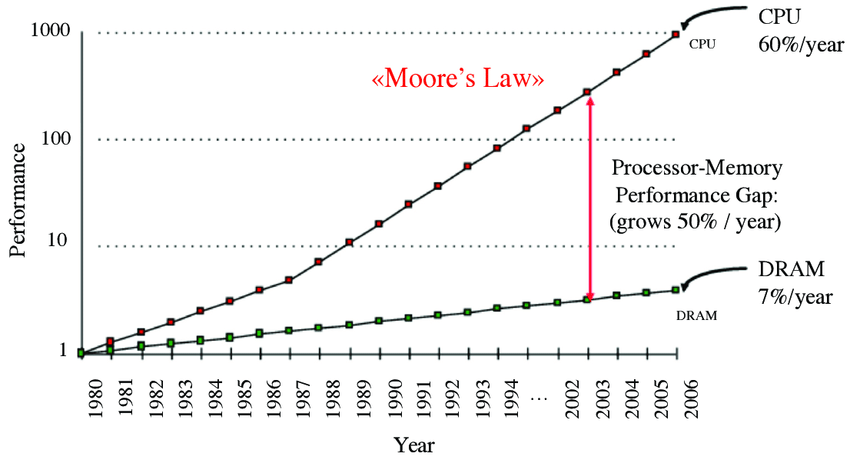
\includegraphics[scale=0.4]{images/CPUvsMEMORY.png}
    \caption{CPU and Memory performance difference over the years [2]}
    \label{fig:cpu-memory}
\end{figure}

% Introduction of DOTS
Finally coming to the conclusion, Data-Oriented Technology Stack (DOTS) in Unity represents a paradigm shift in game development, leveraging Data-Oriented Design (DOD) principles to maximize performance and scalability. Built upon the Entity-Component-System (ECS) architecture, DOTS decouples data and behavior, enabling developers to optimize hardware utilization and minimize overhead. This approach prioritizes efficient data organization and processing, allowing developers to harness the full potential of modern hardware architectures.

Unity DOTS which was for the first time announced in 2018 and production ready released on May 25th 2023 introduces several key components:

\begin{itemize}
    \item \textbf{ECS for Unity} --> This framework provides seasoned Unity creators with greater control and determinism, enabling the creation of more performant games through data-oriented design.
    \item \textbf{Burst Compiler} --> Burst translates IL/.NET bytecode into highly optimized native code, leveraging the industry-proven LLVM compiler infrastructure. This compiler exposes CPU intrinsics, allowing for fine-tuning of performance-critical code.
    \item \textbf{C sharp Job System} --> This system enables developers to leverage multi-core computing platforms by running parallelized code safely and efficiently. By exposing Unity's internal C++ Job System, developers can seamlessly integrate their scripts with Unity's internal processing.
\end{itemize}

Together, these components create a powerful infrastructure for game development, offering enhanced performance, scalability, and maintainability.

While there are other similar solutions available, such as Unreal Engine's ECS and CryEngine's Job System, DOTS stands out due to its tight integration with the Unity ecosystem and its focus on enabling developers to achieve optimal performance and scalability. Its relatively recent release also presents a significant opportunity for exploration and integration into game development projects. Additionally some benefits of using DOTS in games can include scalability in sense of having more stuff happening in a game and possibility of running it on smaller/worst hardware\newline


% How those can complement each other
Summarizing the basic knowledge behing the concepts of DOTS and GGPO we can see that there is some potentiall to get in merging those. DOTS represents a promising avenue for game developers looking to push the boundaries of performance and scalability in their projects. Additionally GGPO can camplement it with seemless lag handling, enabling lockstep architecture and would also use capabilities of DOTS when the sitution of fast resimulation of multiple frames happens.
Additionally there is some probability that reduced CPU cost i.e. higher performance can lead to reduced latency supporting GGPO goal, but only if the CPU + socket poor performance is wasting many milliseconds so it can be an additional benefit. When it comes to direct latency it shouldn't be expected that DOTS + GGPO will reduce it much. Existing GGPO approaches already reduce latency as much as humanly possible. What DOTS + GGPO offers is reduced CPU consumption i.e. higher game scope / scale. It's also potentially easier to work with.



% Additional benefits in different section???

% QUESTIONS
    % 1) Confirm dates for rollback, ggpo and player prediction --> check rollback netcode/client prediction (1996), context of lockstep/ggpo (2008)
    % 2) How much do I need to explain the topic (for example network delay)
    % 3) Correct how I use citations 
    % 4) What are netcode architectures/differences --> There are only a few different types of Netcode architecture, but almost every game will have a unique implementation of one of these architectures. We're using the GGPO architecture (or model)
    % 5) We are planning to do a custom GGPO implementation